\chapter{Technical Details} 
\label{chap:implementation}

This section delves into TimeKeeper's implementation. This section should be read if you plan to modify the TimeKeeper source code. TimeKeeper's implementation can broken up into distinct components: the Linux Kernel modifications, the TLKM, and the integration of TimeKeeper with various network simulators. This chapter will describe each of these components in detail.
\begin{figure}[t] 
      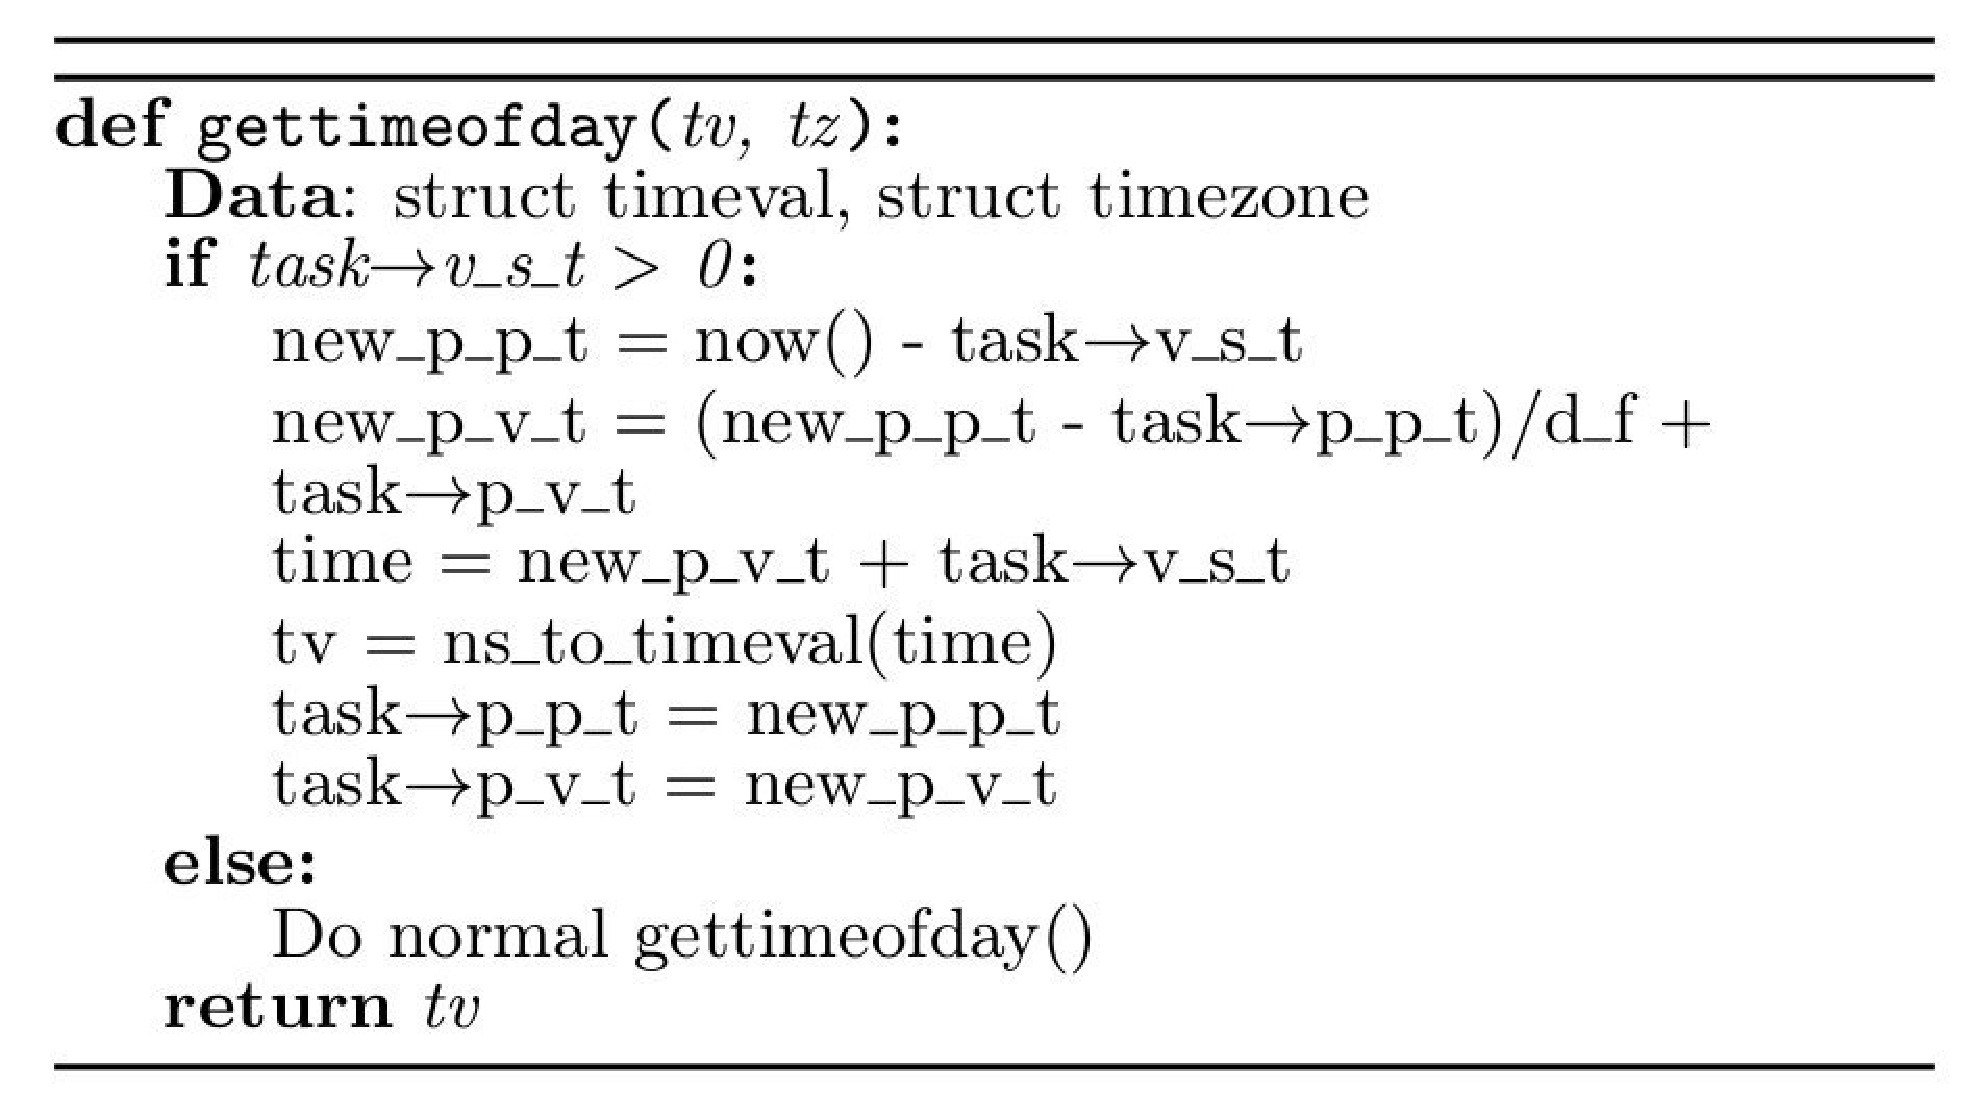
\includegraphics[width=\textwidth]{images/gettimeofday_alg.eps} 
    \caption{Pseudocode For Modified Getttimeofday System Call} 
    \label{fig:gettimeofday_alg} 
  \end{figure} 
\begin{figure}[t] 
      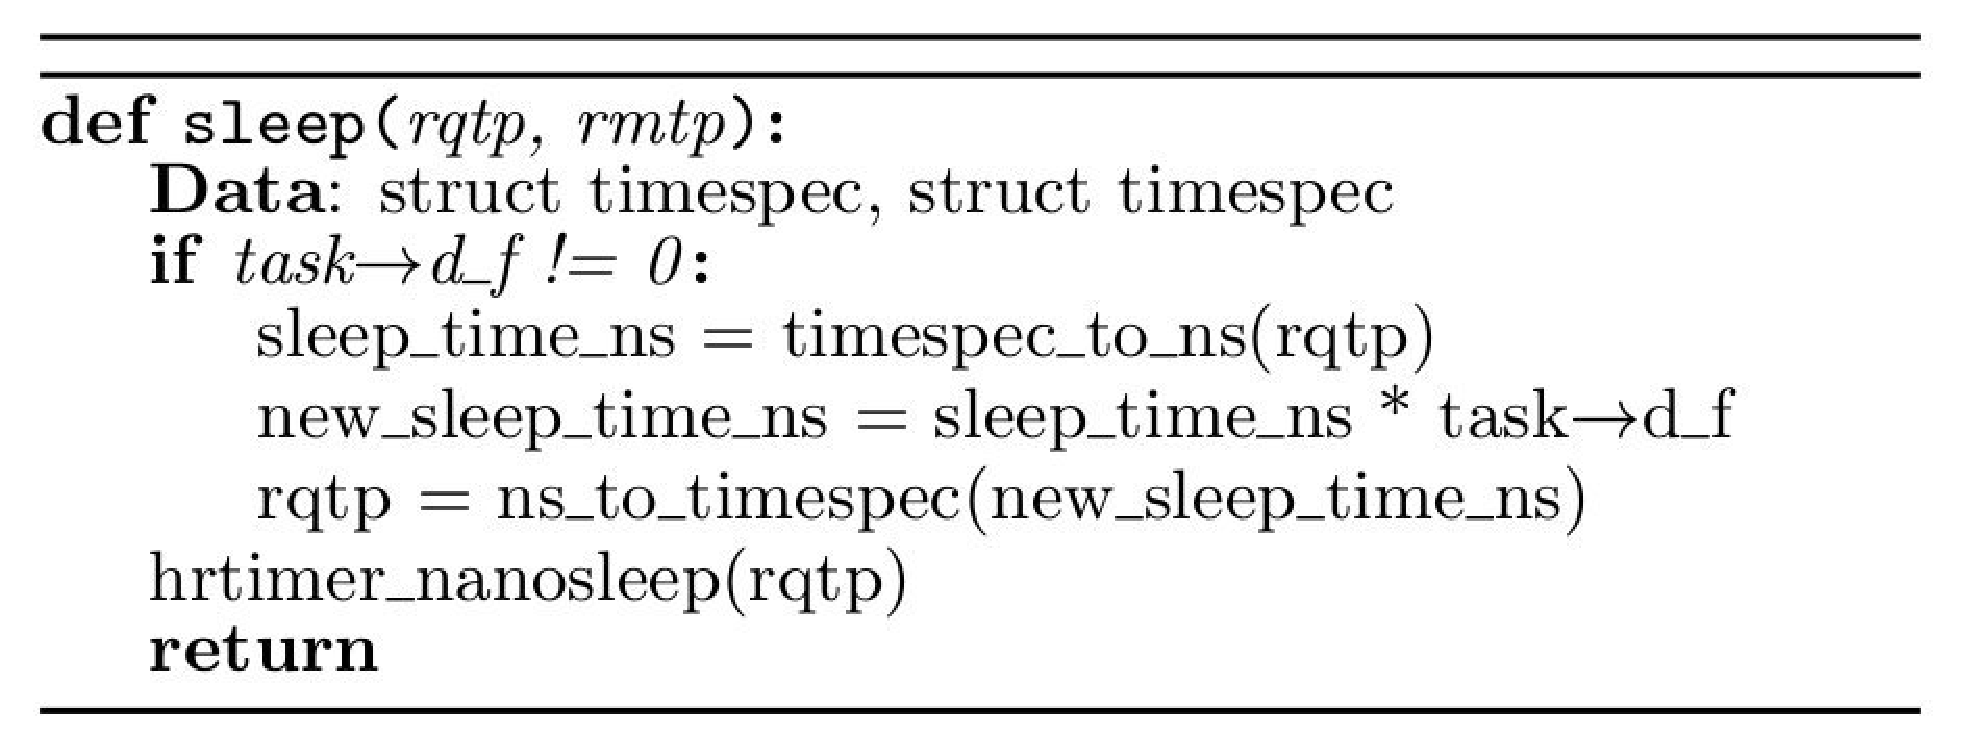
\includegraphics[width=\textwidth]{images/sleep_alg.eps} 
    \caption{Pseudocode For Modified Nanosleep System Call} 
    \label{fig:sleep_alg} 
  \end{figure} 
\section{Kernel Modifications}
\label{sec:kernel_modifications}
In this section, we will discuss the purpose of each modified file in the Linux Kernel, the reason why we needed to modify that particular file, as well as describe the changes made. All of our kernel modifications were made to a 32-bit 3.10.9 Linux Kernel, then extended to work on a 64-bit Linux Kernel as well.
\subsection{32-bit TimeKeeper}
\begin{description} 
\item[linux-3.10.9/include/linux/init\_task.h] \hfill \\
        The $init\_task.h$ file defines many structures having to do with an individual process. Most importantly for us, it initializes all variables in the Linux $task\_struct$ structure. There exists a $task\_struct$ for every running process in Linux, and it maintains important information pertaining to that particular process. It was within this structure where we added six additional variables (44 bytes) in order for each process to maintain its own notion of virtual time. The variables added are:
        \begin{itemize} 
                        \item 4 bytes $dilation\_factor (d\_f)$ represents the TDF of the process. It may be either positive or negative. It is important to realize a TDF is represented as an $integer$ within the Linux Kernel, but as a $float$ from a user's perspective. This is because doing floating point calculations from within the Linux Kernel is very difficult, and it is recommended not be be done. Therefore, when a user supplies a TDF as a float, it will be converted to an integer before it is used in virtual time calculations. This process is completely transparent from the user's perspective.
                \item 8 bytes $virtual\_start\_time (v\_s\_t)$ represents the point in system time (in ns) in which the process started progressing in virtual time by a scaled factor of its TDF.
                \item 8 bytes $past\_virtual\_time (p\_v\_t)$ represents how far virtual time has progressed from the $v\_s\_t$ since the last time the process inquired about the current time.
                \item 8 bytes $past\_physical\_time (p\_p\_t)$ represents how far physical time has progressed from the $v\_s\_t$ since the last time the process inquired about the current time.
                \item 8 bytes $freeze\_time (f\_t)$ is used to determine if the process is currently frozen or not. If the value of $freeze\_time$ is zero, then the process is currently not frozen. If the process is currently frozen, then $freeze\_time$ will be set to the point in time (in ns) in which the process was frozen. This variable is kept entirely internal to TimeKeeper. 
	\item 8 bytes $wakeup_time (w\_t)$ variable is used to ensure the process sleeps for the appropriate amount of time, regardless of whether or not it is in an $experiment$ or not. The need for this variable is further discussed in Section \ref{sec:hooking}.
        \end{itemize}
        How these variables interact with each other to give the process a different perception of time will be explained in later sections. 
\item[linux-3.10.9/linux/kernel/time.c] \hfill 
        \begin{itemize} 
                        \item \textbf{gettimeofday()} \\
                        The $gettimeofday()$ system call allows a user-land process to determine the current system time to within microsecond accuracy. The $gettimeofday()$ system call is one of the only ways for a process to determine the current system time, and it is the most popular method. Therefore, in order to change a process's perception of time, we modify this system call to return a different time from the system time, which is based on the calling process's TDF. See Figure \ref{fig:gettimeofday_alg} for the algorithm. If the process who calls $gettimeofday()$ has its $virtual\_start\_time$ set, then the modified virtual time will be returned. If the process does not have the $virtual\_start\_time$ set, then the normal $gettimeofday()$ function is called, and the system time is returned. \\ \\
Let us consider an example with an LXC with TDF 2 for clarification on the modified $gettimeofday()$ system call. Note this means for every 2 seconds of clock time, the process will perceive only 1 second of virtual time. We assume the process is started at the system time of 20 seconds. At this point in time, $d\_f=2, v\_s\_t=20, p\_v\_t=0, and\ p\_p\_t=0$. Suppose this process performs a computation for 10 seconds, and then calls $gettimeofday()$. Following the pseudocode, a new\_p\_p\_t will be calculated by subtracting the current system time from the v\_s\_t. So the new\_p\_p\_t = 30s - 20s = 10s. A new\_p\_v\_t is then calculated by finding the time which has elapsed since the last past\_physical\_time, scaling it appropriately based on the TDF, and finally adding it to the last past\_virtual\_time. Thus, new\_p\_v\_t = (new\_p\_p\_t - p\_p\_t)/d\_f + p\_v\_t = (10s - 0s)/2 + 0 = 5s. So the virtual\_time = v\_s\_t + new\_p\_v\_t = 25 seconds, which is the correct virtual time for the described scenario. Note, before $gettimeofday()$ returns, new\_p\_p\_t and new\_p\_v\_t are stored into p\_p\_t and p\_v\_t respectively. At the end of this function, the state of the process is: $d\_f=2, v\_s\_t=20s, p\_p\_t=10s, and\ p\_v\_t=5s$ and the global time is 30s. Now assume the process runs for an additional 20 seconds, and checks its time once again. new\_p\_p\_t = 50s - 20s = 30s and new\_p\_v\_t = (new\_p\_p\_t - p\_p\_t)/d\_f + p\_v\_t = (30s - 10s)/2 + 5 = 15s. So the virtual\_time returned is 20s+15s = 35s. As you can see, this is consistent with what is expected, as the process was started at 20 seconds, and has been running with a TDF of 2 for 30 seconds of physical time.
        \end{itemize}
\item[linux-3.10.9/linux/kernel/hrtimer.c] \hfill 
        \begin{itemize} 
                        \item \textbf{nanosleep} \\ 
                        It is not enough to simply modify the $gettimeofday()$ system call to accurately model a process to run with a different perception of time. Within the Linux Kernel, there exist numerous system calls which depend on a consistent notion of scaled time dilation in order to perform accurately and reliably. The $nanosleep()$ system call is one such example. Whenever a process wishes to relinquish its time on the processor and sleep for a specified period of time, $nanosleep()$ is the system call that gets executed. When the $nanosleep()$ system call is called, it will set a high-resolution timer ($hrtimer$) to fire at point in time in the future, where the process will get woken up and allowed to be ran on the processor once again. Suppose we did not modify the $nanosleep()$ system call, and there is a process with a TDF of 2 and wanted to sleep for 5 seconds. It would wake up after 5 seconds of system time has passed, but if it checked the current system time it would find only 2.5 seconds has passed. This is obviously not right, as the program asked to sleep for 5 seconds. Thus, we need to appropriately scale the amount of time the process sleeps by looking at its TDF. In regards with the example, the process would need to sleep for 10 seconds of physical time in order to perceive a change of 5 seconds in virtual time. See Figure \ref{fig:sleep_alg} for the modified pseudocode. 
        \end{itemize}
\item[linux-3.10.9/arch/x86/syscalls/syscall\_32.tbl] \hfill \\
        The $syscall\_32.tbl$ file contains information regarding system calls within the 32-bit Linux Kernel. It contains the number of the system call, its name, and entry point. Since we created two additional system calls to the Linux Kernel, we will need to add the required information to this table. This is required as the Linux kernel needs to know how to call our new system call from a user-land process. The TimeKeeper patch implements two additional system calls: $gettimeofdayreal()$ and $gettimepid()$. They are fully described in Section \ref{subsec:new_system_calls}.
\item[linux-3.10.9/include/linux/sched.h] \hfill \\
The $sched.h$ file defines the Linux $task\_struct$. It declares all variables within the Linux $task\_struct$. It is here where we declare the five additional variables that are associated with every $task\_struct$ to allow for time-dilation: $dilation\_factor$, $virtual\_start\_time$, $past\_virtual\_time$, $past\_physical\_time$, and $freeze\_time$. 
\item[linux-3.10.9/include/linux/syscalls.h] \hfill  \\
The $syscalls.h$ file declares all non architecture specific system calls. This is where we declare the function definitions for the $gettimeofdayreal()$ and $gettimepid()$ system calls. 
\end{description}
\subsection{64-bit TimeKeeper}
\label{subsec:vdso}
A couple steps were necessary to convert 32-bit TimeKeeper to the 64-bit equivalent. 
\begin{description} 
\item[Bypassing the vDSO] \hfill \\
        The virtual dynamic shared object (vDSO) is a small library provided by the Linux Kernel which is mapped into the every single user-space application's address space. The user does not have any direct interaction with the vDSO, as all of the interaction is handled by the C library. The vDSO exists because making system calls can be a slow process. For example, the $gettimeofday()$ system call requires a software interrupt, context switching overhead, as well as writing data from kernel-space to user-space. All of this overhead does not entirely make sense, as a process with any privilege mode on the system can acquire the current system time information. Thus, on newer 64-bit Linux systems, the Kernel places this information in the vDSO, and the process can access it via a few memory accesses as opposed to an actual system call. 

With the vDSO in place, whenever $gettimeofday()$ is called, our modified code is never actually executed. This is problematic, as the process will no longer have a time-dilated view of time. To overcome this, two files were modified in order to force $gettimeofday()$ calls to actually perform the system call. This introduced a fair amount of overhead, which is explored in Section \ref{sec:expvdso}.
\item[linux-3.10.9/arch/x86/syscalls/syscall\_64.tbl] \hfill \\
The $syscall\_64.tbl$ file contains information regarding system calls within the 64-bit Linux Kernel. It is important to know there is a different number of system calls in 32-bit and 64-bit Linux. Therefore,   the additional system calls TimeKeeper provides will be assigned to different numbers. 
\item[linux-3.10.9/arch/x86/vdso/vdso.lds.S] \hfill \\
        In order to have the actual $gettimeofday()$ system call get executed, $vdso.lds.S$ needed to be modified. The file acts as the linker script for the vDSO. It defines any user-exported symbols in the vDSO. Originally, it exports $clock\_gettime()$, $getcpu()$, $gettimeofday()$, and $time()$. The file was modified, and any references of the $gettimeofday()$ system call were removed. This results in the execution of the modified $gettimeofday()$ system call.
\item[linux-3.10.9/arch/x86/vdso/vdsox32.lds.S] \hfill \\
        Same description as above, but for 32-bit Linux. Once again, the $gettimeofday()$ system call was removed, so the actual system call code would be executed.
\end{description}
\subsection{New System Calls}
\label{subsec:new_system_calls}
The TimeKeeper Kernel patch introduces two additional system calls: $gettimeofdayreal()$ and $gettimepid()$. They will be discussed individually. 
\begin{description} 
\item[gettimeofdayreal(struct timeval *tv, struct timezone *tz)] \hfill \\
The $gettimeofdayreal()$ system call will return the actual system time, regardless if the container has a TDF or not. The code is exactly the same as the original $gettimeofday$ system call. The system call was originally implemented to ensure the modified $gettimeofday()$ was returning appropriate results. Users of TimeKeeper may take advantage of this system call for the same reason.   
\item[gettimepid(pid\_t pid, struct timeval *tv, struct timezone *tz)] \hfill \\
The $gettimepid()$ system call allows you to query the virtual time of a particular container. For example, you may be running two containers at different TDFs, thus their virtual times to be different. If you know the pids of both containers, you can query each container's virtual time individually. The system call was implemented in order to properly integrate TimeKeeper with the S3F network simulator. 
\end{description}
\section{Kernel Module}
\label{sec:kernel_module}
        TimeKeeper can perform simple time dilation with only the modifications to the kernel. However, more advanced features such as the ability to freeze and unfreeze a process' advancement in virtual time, or group multiple processes with different TDF's together to have their virtual times advance uniformly in time was not put directly into the Linux kernel. Instead, these features were developed in the form of a Linux Kernel Module (LKM) which may be loaded into the Linux kernel at run time. The LKM performs two advanced features: individual process freezing/unfreezing, and experiment synchronization. These features will be discussed separately. 
\subsection{Freezing/Unfreezing}
\label{subsec:freezing_unfreezing}
        In order to $freeze$ or $unfreeze$ a process's perception of time, TimeKeeper makes use of a variable that was added to each process's $task\_struct$: $freeze\_time\ (f\_t)$. If the user wishes to $freeze$ a process, its $f\_t$ is set to the current, non-dilated system time, and a SIGSTOP signal is sent to the process. A SIGSTOP signal is built into the Linux Kernel, and tells the process to remove itself from running on the current processor until further notice. When the user wishes to $unfreeze$ a previously frozen process, the process's $p\_p\_t$ is updated to reflect the amount of physical time in which the process was frozen $(p\_p\_t =  p\_p\_t + (current\_system\_time\ $–$\ f\_t))$. Immediately after, a SIGCONT signal is sent to the process. The SIGCONT signal is also built into the Linux Kernel, and allows the process to continue execution on a processor. Then, $f\_t$ is set to zero, and the process is officially unfrozen. \\
Let us continue the example from the previous section, and assume the process was frozen immediately after it last checked its time (virtual\_time=35s, system\_time=50s). The current state of the process is: $d\_f=2, v\_s\_t=20s, p\_p\_t=30s, p\_v\_t=15s, f\_t=50s$. The process is first frozen for 10 seconds, then unfrozen and immediately checks the time. When it is unfrozen, the $p\_p\_t$ is changed to $(p\_p\_t + (current\_system\_time - f\_t)) = (30s + (60s-50s)) = 40s$. When it checks the time with the updated $p\_p\_t$ value, it returns 35s, therefore not recognizing any time has passed since it was frozen. See Figure \ref{fig:freeze_alg} and Figure \ref{fig:unfreeze_alg} for freezing and unfreezing psuedocode respectively. 
\begin{figure}[t] 
      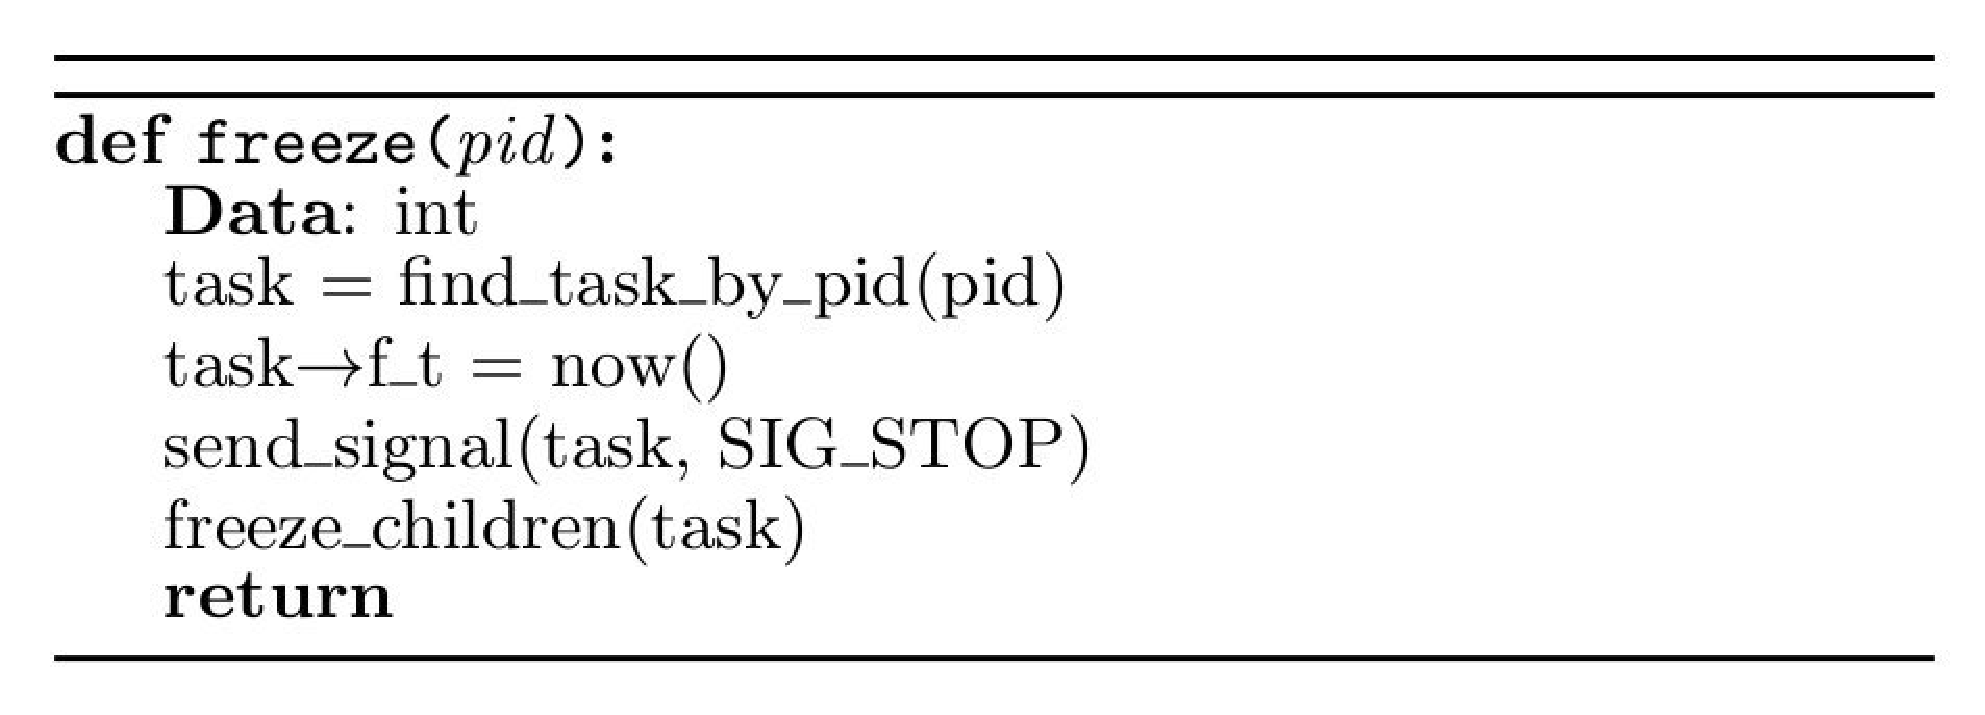
\includegraphics[width=\textwidth]{images/freeze_alg.eps} 
    \caption{Pseudocode For Freeze Functionality} 
    \label{fig:freeze_alg} 
  \end{figure} 
\begin{figure}[t] 
      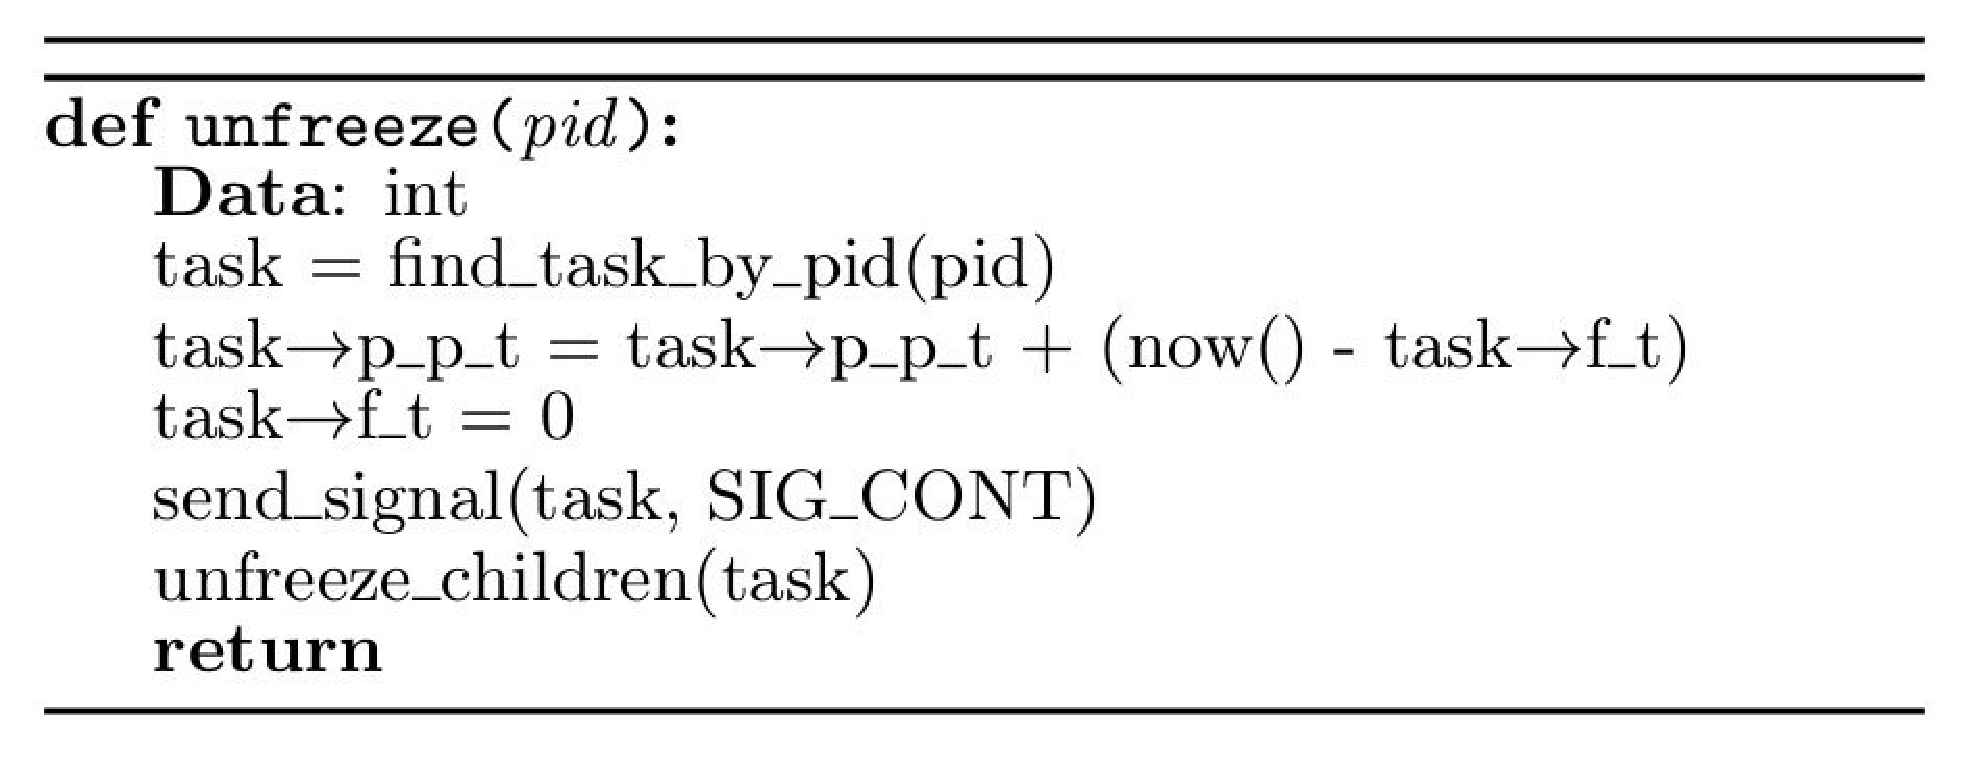
\includegraphics[width=\textwidth]{images/unfreeze_alg.eps} 
    \caption{Pseudocode For Unfreeze Functionality} 
    \label{fig:unfreeze_alg} 
  \end{figure} 
\subsection{Experiment Synchronization}
\label{subsec:experiment_synchronization}
        The TLKM is also capable of grouping processes with different TDFs together into a single $experiment$, where all of the processes virtual times progress uniformly. 
        In order to do this, TimeKeeper maintains a linked list of all processes in the experiment, an adjustable knob called $EXP\_CPU$, and another adjustable knob called a $timeslice$. $EXP\_CPU$ specifies how many processors you are willing to dedicate to the $experiment$. A higher $EXP\_CPU$ value will allow the the $experiment$ to run faster and complete in a shorter amount of physical time. A lower $EXP\_CPU$ value will make the experiment take longer to complete, but more resources will be available for other tasks. In our experiments, we would set $EXP\_CPU$ to be two processors less than the total number of processors on the system. This allows standard background tasks to still be able to run successfully, even if a CPU-intensive experiment is being conducted. The $timeslice$ variable specifies the amount of physical time in which the $leader$ process is allowed to run for each round of the experiment. When an $experiment$ is initialized, TimeKeeper will determine the $leader$, which is the process with the highest TDF. Knowing the $leader$ is a necessity, as the $leader's$ virtual time will progress slower than any other process in the experiment (because it has the highest TDF). Therefore, TimeKeeper needs to scale down the running time of all other processes in the experiment accordingly. See Table \ref{table:cpufraction} for how the $leader's$ TDF affects the running time of other processes in the experiment. 
\begin{table} \centering 
\begin{tabular}{|c|c|c|c|} 
        \hline 
         & TDF 2 & TDF 1 & TDF .5  \\ \hline 
        Leader TDF 10 & 1/5 & 1/10 &  1/20 \\ \hline 
        Leader TDF 5 &  2/5 & 1/5 & 1/10 \\ \hline 
        Leader TDF 2 & 1 & 1/2 & 1/4 \\ \hline 
        Leader TDF 1 & x &  1 & 1/2 \\ \hline 
        \hline 
        \end{tabular} 
        \caption{How Leader's TDF Affects other LXCs Fraction of CPU Time} 
        \label{table:cpufraction} 
\end{table}
For example, consider a $leader$ with a TDF of 2, and another process with a TDF of 1. In order to keep these processes' virtual times synchronized, the process with a TDF of 1 will need to run for one half the time in which the $leader$ is allowed to run. 
\begin{figure}[t] 
      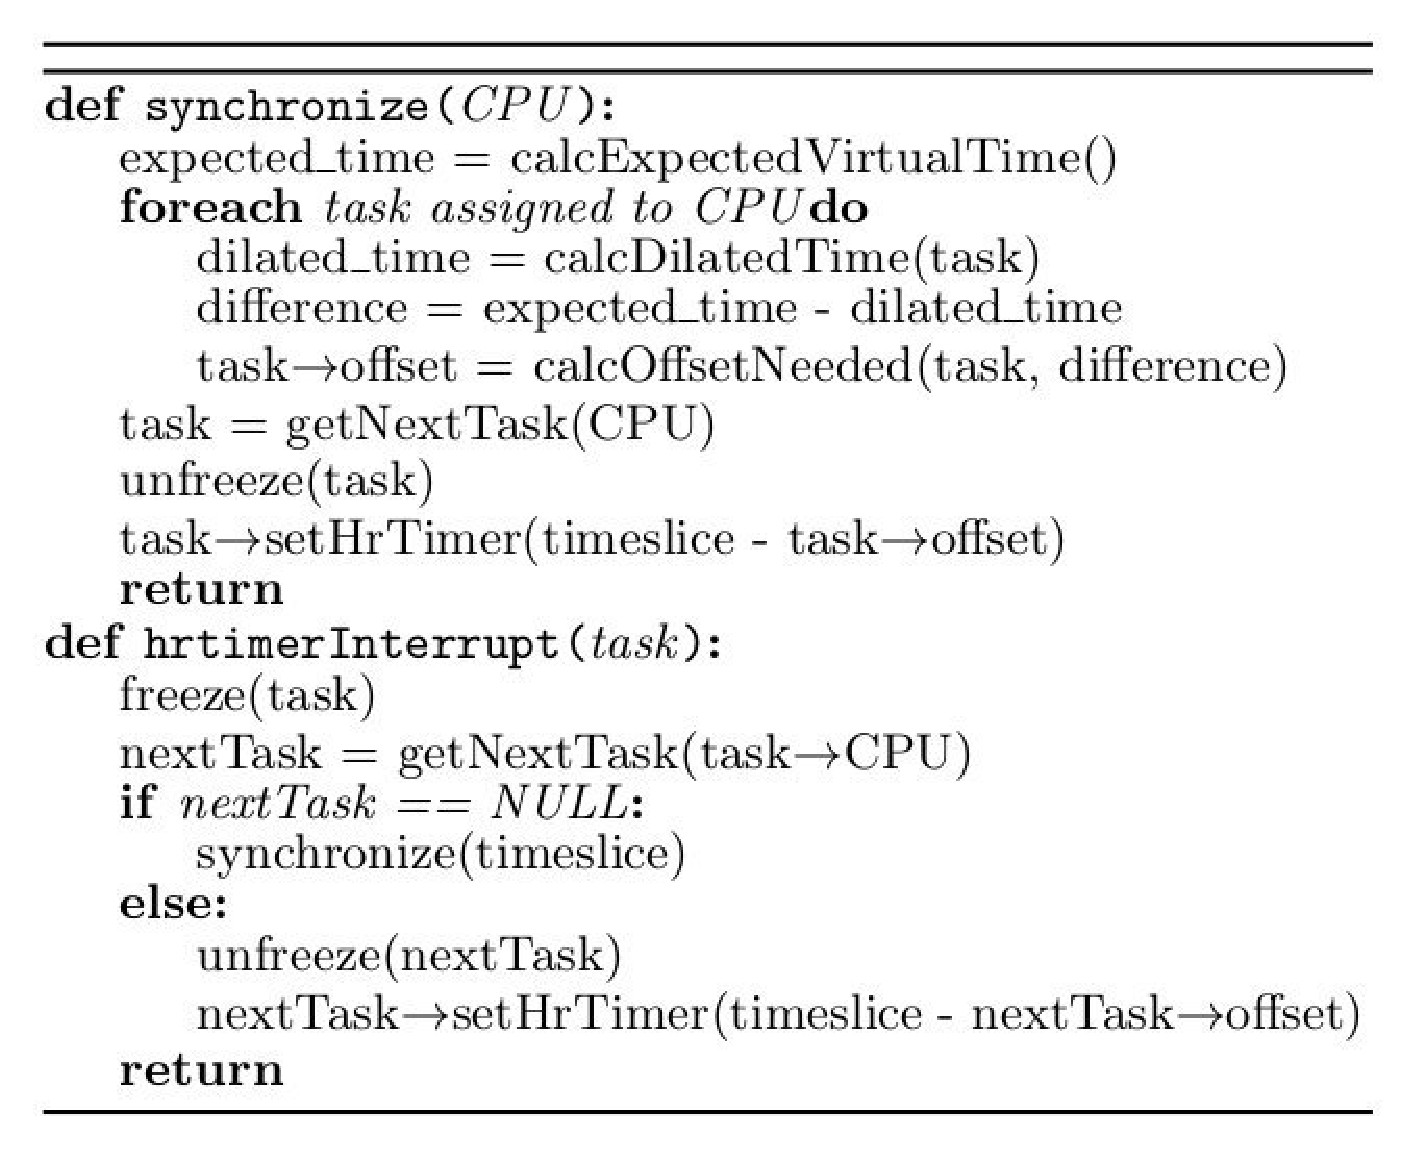
\includegraphics[width=.9\textwidth]{images/synchronization_alg.eps} 
    \caption{Pseudocode For LXC Synchronization Algorithm } 
    \label{fig:synchronization_alg} 
  \end{figure} 
        Once the $leader$ has been appointed, each process in the experiment is dedicated to a specific processor, where multiple processes may be mapped to the same processor, and set to have a scheduling policy of SCHED\_FIFO (first-in first-out). A SCHED\_FIFO scheduling policy allows the process to have a higher priority than other tasks not in the experiment, as well as not get preempted until TimeKeeper decides the process should no longer be allowed to run. Then, each process will be allocated a fraction of the $timeslice$ in which it will be allowed to run on its dedicated processor for each round. This fraction of the $timeslice$ is based on the process's TDF with respect to the $leader's$ TDF, and maintained by a high-resolution timer ($hrtimer$). At the beginning of each round of the experiment, all processes are in the $frozen$ state. For each dedicated CPU a process is chosen to run, and it is unfrozen with TimeKeeper's previously mentioned $unfreeze$ capability. When the process is unfrozen, its respective $hrtimer$ is set to expire when its predetermined fraction of the $timeslice$ is up. When the $hrtimer$ for the process expires, the process is frozen, and the next process whose turn it is to run on the CPU is unfrozen and has its $hrtimer$ set. This process continues until all processes in the $experiment$ have been allowed to run for their fraction of the $timeslice$. When all processes in the $experiment$ have ran, the round is up. At the beginning of each round, a new $leader$ may be calculated if the current $leader$ finished executing, if new processes with higher TDFs were added to the experiment, of if a process in the experiment had its TDF changed to be higher than the current $leader$. In addition, a simple check will be done for each process to determine if it should run a little longer or little less in the following round. This is done by comparing each process's virtual time to the expected virtual time of the experiment. If the process's virtual time exceeds the expected virtual time of the experiment, that process will be forced to run for less time in the current round (by setting its $hrtimer$ to fire sooner). If a process's virtual time is below the expected virtual time of the experiment, that process will be allowed to run for more time in the current round (by setting its $hrtimer$ to fire later). When all processes know how long they can run for the current round, the round may continue. See Figure \ref {fig:synchronization_alg} for the psuedocode for the synchronization algorithm.
\subsection{Hooking the System Call Table}
\label{sec:hooking}
The TLKM also needs to hook the system call table in order to ensure certain system calls like $sleep()$ behave appropriately when called from a process within a synchronized experiment. The modified $sleep()$ system call as referenced in Section \ref{sec:kernel_modifications} will work correctly if the calling process is running independently, because you can simply look at the process's TDF. However, if the calling process is within a synchronized experiment, the virtual time will be advancing at the rate of the leader's TDF, not the calling process's TDF. Therefore, the process will need to be awoken when the experiment's virtual time reaches the wake up point. To determine this point, the $sleep()$ system call is replaced dynamically with our own function when the TLKM is loaded into the Linux Kernel. The new function will first determine if the calling process is within a synchronized experiment. If it is not, it will perform the regular $sleep()$ system call. If the process is within a synchronized experiment, it will be put to sleep, and set to resume execution when the experiment's virtual time surpasses the wake up time. When the TimeKeeper Kernel Module is removed from the Linux Kernel, the $sleep()$ system call is unhooked and returned to its regular functionality.

\section{CORE Integration}
CORE is capable of emulating the networking stack of various routers and end hosts through virtualization and then simulating the links between such devices. CORE was chosen as the initial system to be integrated with TimeKeeper because it uses network namespaces to divide processes into logically separate networking entities (giving each process its own routing tables, network adapters, and so forth). Internally, LXCs use network namespaces to achieve the same goal. However, LXCs provide additional features, such as the ability to create persistent containers via configuration files, or resource isolation via cgroups. CORE does not need the advanced features of LXCs, so the simpler network namespace alternative was used. Because LXCs are so closely tied to network namespaces, it made CORE an ideal first system to integrate with TimeKeeper. The next two sections will give an overview of how CORE works under the hood, followed by a description of the necessary changes made for the TimeKeeper integration. 
\subsection{CORE Subsystem Overview}
CORE consists of two major components: a Tcl/Tk GUI frontend, and a CORE daemon backend. The CORE daemon listens on a local TCP port for specific messages (known as the CORE API) from the graphical user interface (GUI), giving it commands to create specific topologies. To help illustrate what is going on behind the scenes, I will use a simple 2-node example as shown in Figure \ref{fig:core2node}. 
\begin{figure}[t] 
      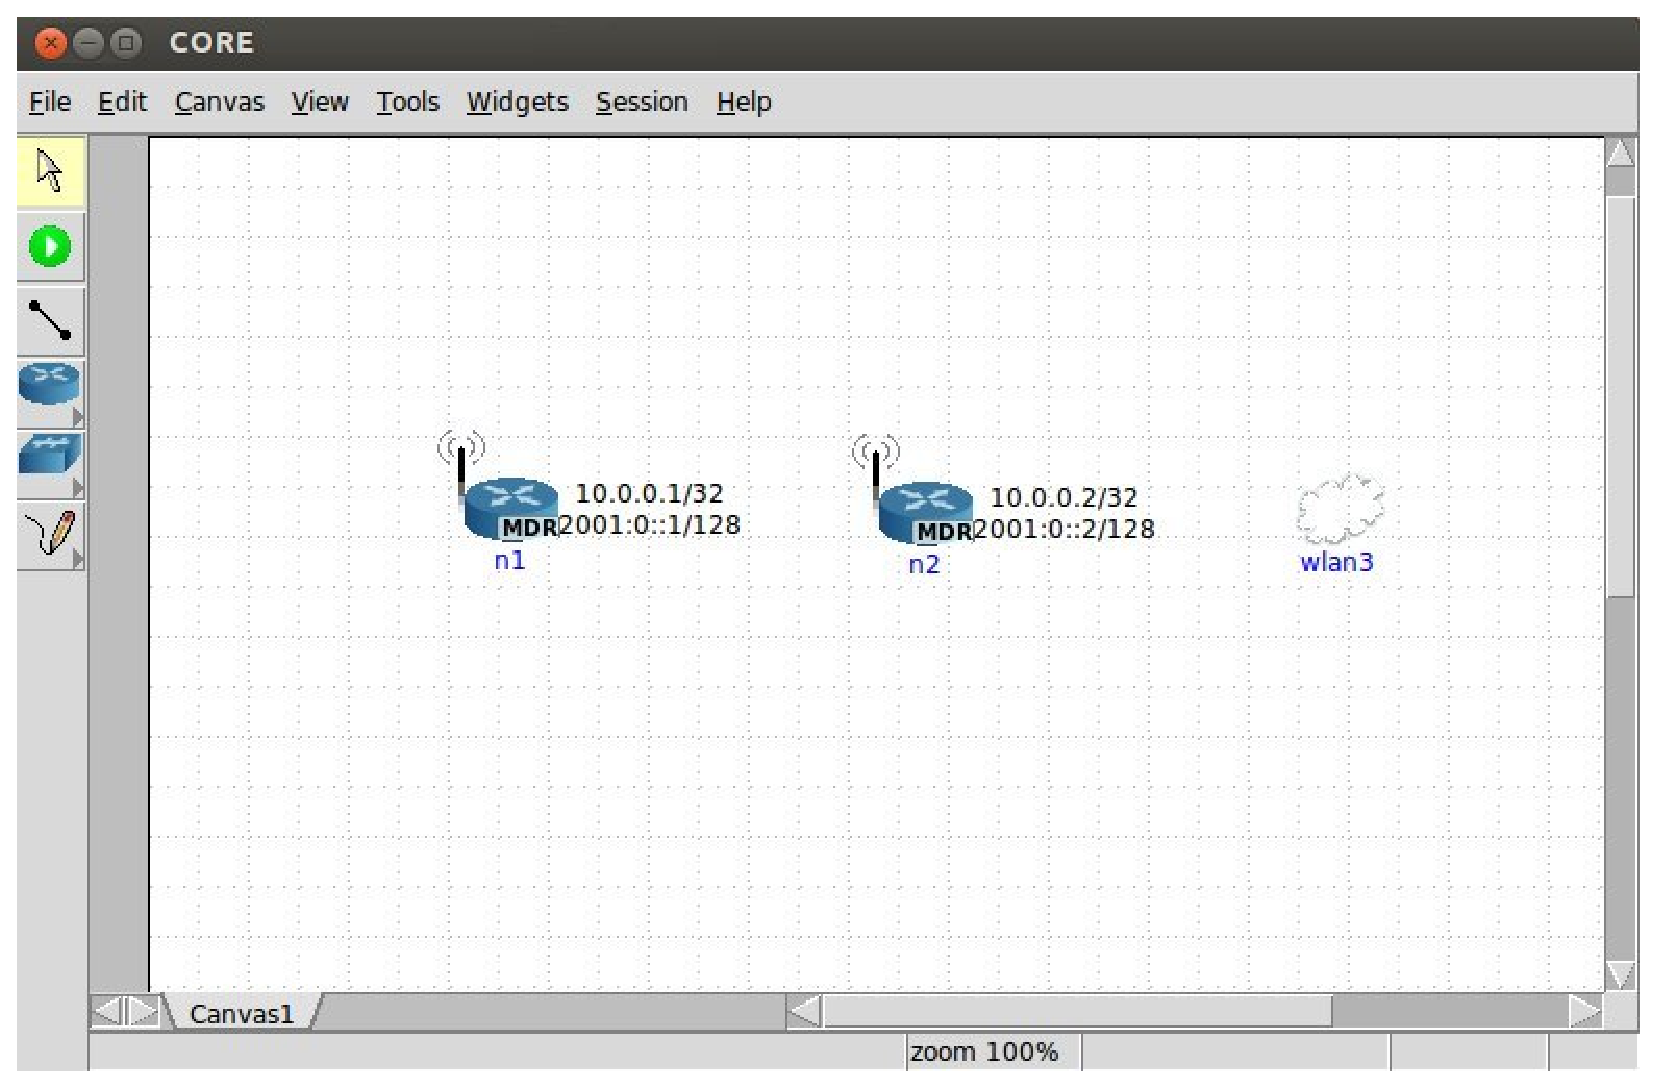
\includegraphics[width=\textwidth]{images/core2node.eps} 
    \caption{Simple 2-Node Topology in CORE} 
    \label{fig:core2node} 
  \end{figure}
This example will model basic on/off wireless connectivity. If the two routers are close enough (as determined by the physical distance from one another in the CORE GUI), they will be able to communicate, if the routers are too far away they will not be able to communicate. The experiment will be started when the green play button is clicked from within the GUI. When this action occurs, the GUI will send all necessary messages describing the created topology to the CORE daemon. For every node in the topology (router or host), the GUI will send a $Node Message$ to the CORE daemon, which will spawn a $vnoded$ daemon responsible for creating its own network namespace. To establish the connectivity, CORE will use a combination of virtual Ethernet pair drivers ($veth$), Linux Bridging, and Ethernet Bridging Tables (ebtables). A $veth$ is simply a Ethernet-like device that can be used inside of a container. Each $veth$ consists of two Ethernet devices, one of which will be installed on the host, while the other will be installed inside the newly created container. When a packet is sent to one of the devices, it will simply come out the other device. The appropriate $veth's$ will then be tied together with Linux bridges. You may think of a Linux bridge as a switch. Finally, appropriate $ebtable$ rules will be applied to the bridge, determining if packets should be dropped or not, depending on the physical distance between the containers. See Figure \ref{fig:coreInternals} to see how two containers are connected in CORE.
\begin{figure}[t] 
      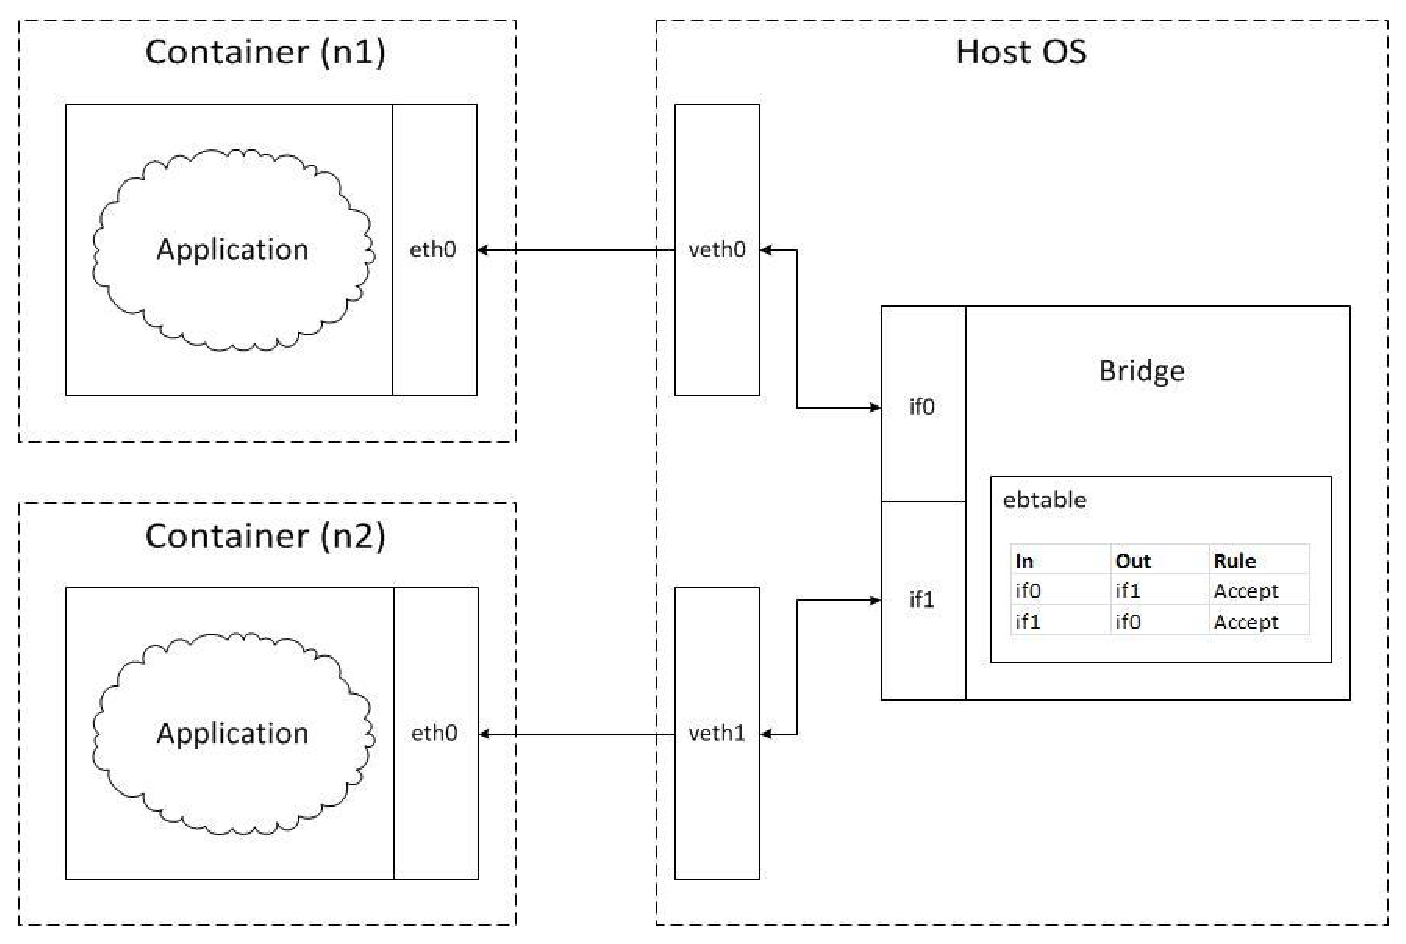
\includegraphics[width=\textwidth]{images/coreInternals.eps} 
    \caption{Connecting Two Containers Within CORE} 
    \label{fig:coreInternals} 
  \end{figure}
\subsection{CORE Modifications}
In order to integrate TimeKeeper with CORE, only a few changes had to be made. Modifications had to be made to allow both the GUI and $vnoded$ daemon to communicate with TimeKeeper. These modifications are illustrated below, and accompanied with a flowchart depicting the changes (see Figure \ref{fig:coreContainerCreation}). 
\begin{enumerate}
        \item First, the GUI was modified in order to maintain additional topology information, and provide the means for the user to input additional information. Now, if a user double clicks on a entity, the option is provided to set that entities TDF. Alternatively, the user could set the TDF of every entity in the window from the 'Tools' tab. The GUI maintains state information for every entity in the window, so when the TDF is set for an entity, its corresponding dilation variable is set appropriately. 
        \item When the topology is constructed, the user clicks the green play button to start the experiment. When this button is clicked, one thing the GUI will do is traverse $node\_list$, which is a list of every node in the GUI. For every node, a “Node Message” which contains information for that node will be sent to CORE daemon. The “Node Message” contains a field called 'opaque' which is meant for user-defined data. Each entities TDF is passed to the CORE daemon via this 'opaque' field.
        \item The CORE daemon receives each “Node Message”, and handles it with the $handlenodemsg$ function. The function extracts the necessary information from the “Node Message”, including the TDF. Then, a modified $vnoded$ script is called. This modified script is able to accept an additional command line argument, the TDF of the container.
        \item The $vnoded$ script calls $nsfork$, which actually creates the network namespace via a $clone()$ system call. The $nsfork$ function was modified so once the $clone()$ system call returns, the new container immediately gets assigned its TDF. Before $nsfork$ returns, it sends the PID of the new container to TimeKeeper. This tells TimeKeeper to add the new container to the synchronized experiment. 
        \item After a short time, all of the time-dilated containers will be set up, and the CORE experiment will begin. From this point, the user may tell TimeKeeper to start the experiment in order to have all the containers virtual time progress uniformly through time. This can be done through the 'Tools' tab, which will send the start message to TimeKeeper. 
\end{enumerate}

\begin{figure}[t] 
      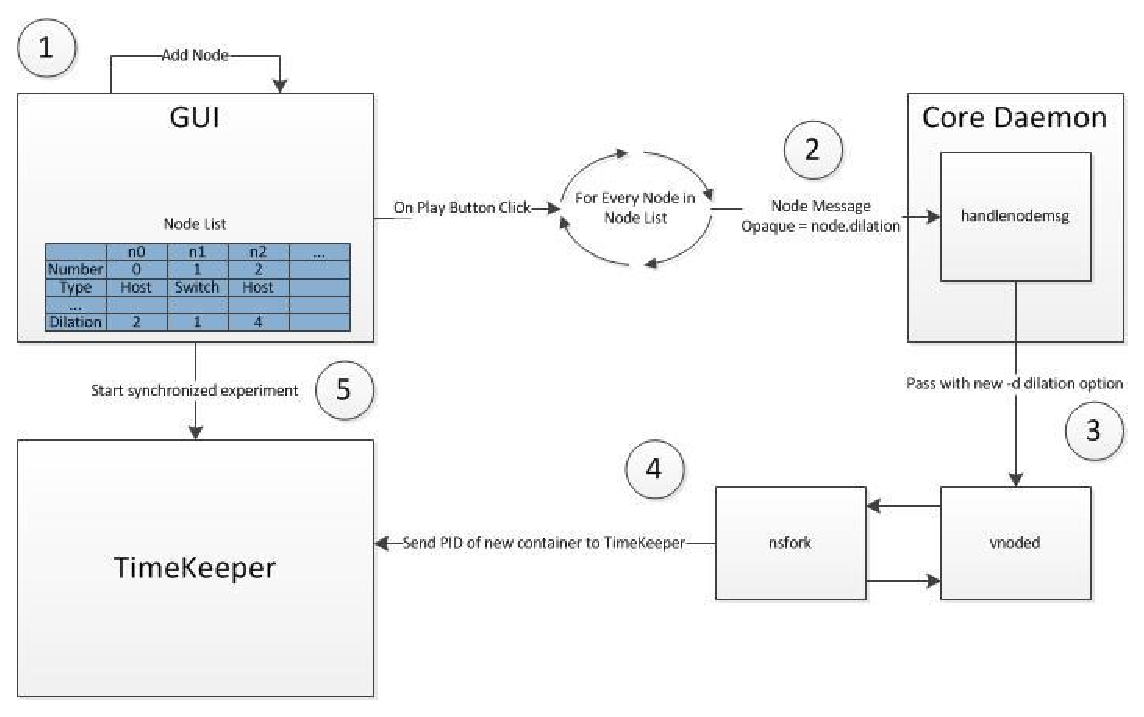
\includegraphics[width=\textwidth]{images/coreContainerCreation.eps} 
    \caption{Core Modifications To Support TimeKeeper} 
    \label{fig:coreContainerCreation} 
  \end{figure}

\section{NS-3 Integration}
NS-3 is an extremely popular discrete-event network simulator, designed primarily for research or educational use. It is composed of numerous 'network' models, such as Wi-Fi or LANs. We are particularly interested in ns-3's ability to interact with real systems, for 'simulation-in-the-loop' experiments. This is done with a RealTime Scheduler. The following two sections will give a brief overview of how ns-3 works under the hood, followed by a description of the necessary changes made for TimeKeeper integration. 
\subsection{NS-3 Subsystem Overview}
Describing all of the components composing ns-3 would be out of the scope of this paper. Instead, we will focus on the components that allow us to hook LXCs to the ns-3 simulator: the RealTime Scheduler and the TapBridge Model. The will be discussed separately.
\begin{itemize} 
                        \item \textbf{RealTime Scheduler} \\ 
                        The default scheduler for ns-3 is not realtime. In this case, when an event is processed, the simulator's time will jump to the time of the next scheduled event. Obviously, this technique will not work if ns-3 is tied to an external entity, as it may send a network packet at any time. If the simulation clock is jumping far ahead, it will not process this packet correctly. Thus, the RealTime Scheduler was implemented, which attempts to keep ns-3's simulation clock synchronized with respect to an external time base (most commonly the wall clock). The RealTime Scheduler works as follows: When the next event in the simulation is ready to be processed, the scheduler will compare the system clock with the scheduled time of the event. If the scheduled time of the event is close to the system clock, it will get executed. If the scheduled time of the event is in the future, the simulator will sleep until the system clock catches up to the scheduled time of the event, then execute that event. It is also possible for the simulator to fall behind the system clock (if the simulator can not process a series of events fast enough). For when this happens, the scheduler has two options, which the user can specify: BestEffort or HardLimit. If the scheduler is running in BestEffort, it will repeatedly process events until it is able to catch up to the system clock. It may never be able to catch up to the system clock if the simulator is constantly overloaded with events. The HardLimit option will also try to catch up to the system clock, but will end the simulation if the difference between the system clock and the simulation clock becomes too large. See Figure \ref{fig:realtimeScheduler}.

\begin{figure}[t] 
      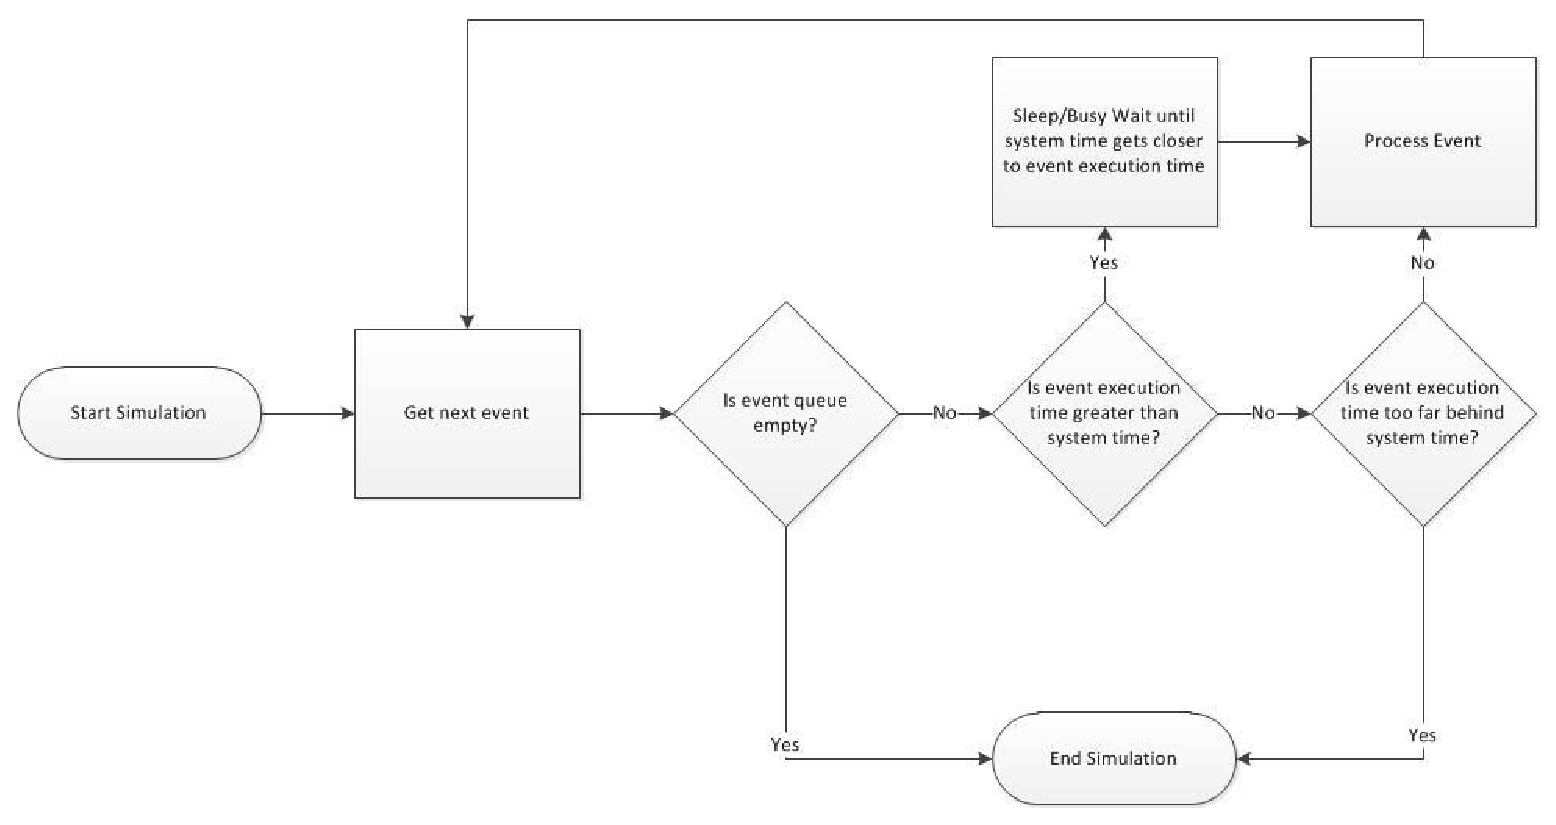
\includegraphics[width=\textwidth]{images/realtimeScheduler.eps} 
    \caption{Simplified NS-3 Flowchart with Realtime Scheduler} 
    \label{fig:realtimeScheduler} 
  \end{figure}
                \item \textbf{TapBridge Model} \\ 
                        The TapBridge Model was designed to integrate real internet hosts (LXCs) with an ns-3 simulation. It works by essentially connecting the inputs and outputs of a Linux TAP device with the inputs and outputs of an ns-3 Net Device. A Linux TAP device allows for user space programs to send and receive packets without needing to traverse physical media. The Linux TAP acts as the glue connecting an LXC and the ns-3 simulation. In ns-3, the Net Device is an abstraction which covers the simulated hardware as well as the software driver. It can be installed on a 'Node', which enables the Node to communicate with others in the simulation. For every real internet host (or LXC) we wish to integrate into the ns-3 simulation, the TapBridge Model will create a 'Ghost Node'. A Ghost Node is simply a Node that is representing an external entity (where the upper levels are not being simulated). For every TapBridge on the Ghost Node there is a corresponding ns-3 NetDevice in which it is acting as the bridge. Everytime the LXC sends a packet, the TAP Device will bring it into user-space, modify the MAC addresses appropriately, and forward it to the Net Device. Likewise, when a packet is received on a ns-3 NetDevice, the TapBridge will grab it, modify the MAC addresses, and send it out the TAP Device. The MAC addresses within packets need to be modified because the TAP Device and ns-3 NetDevice have different MAC addresses. This MAC address spoofing will make it appear for the LXC to have the ns-3 NetDevice as a local device. See Figure \ref{fig:ns3internals} for how LXCs are connected to ns-3.
\begin{figure}[t] 
      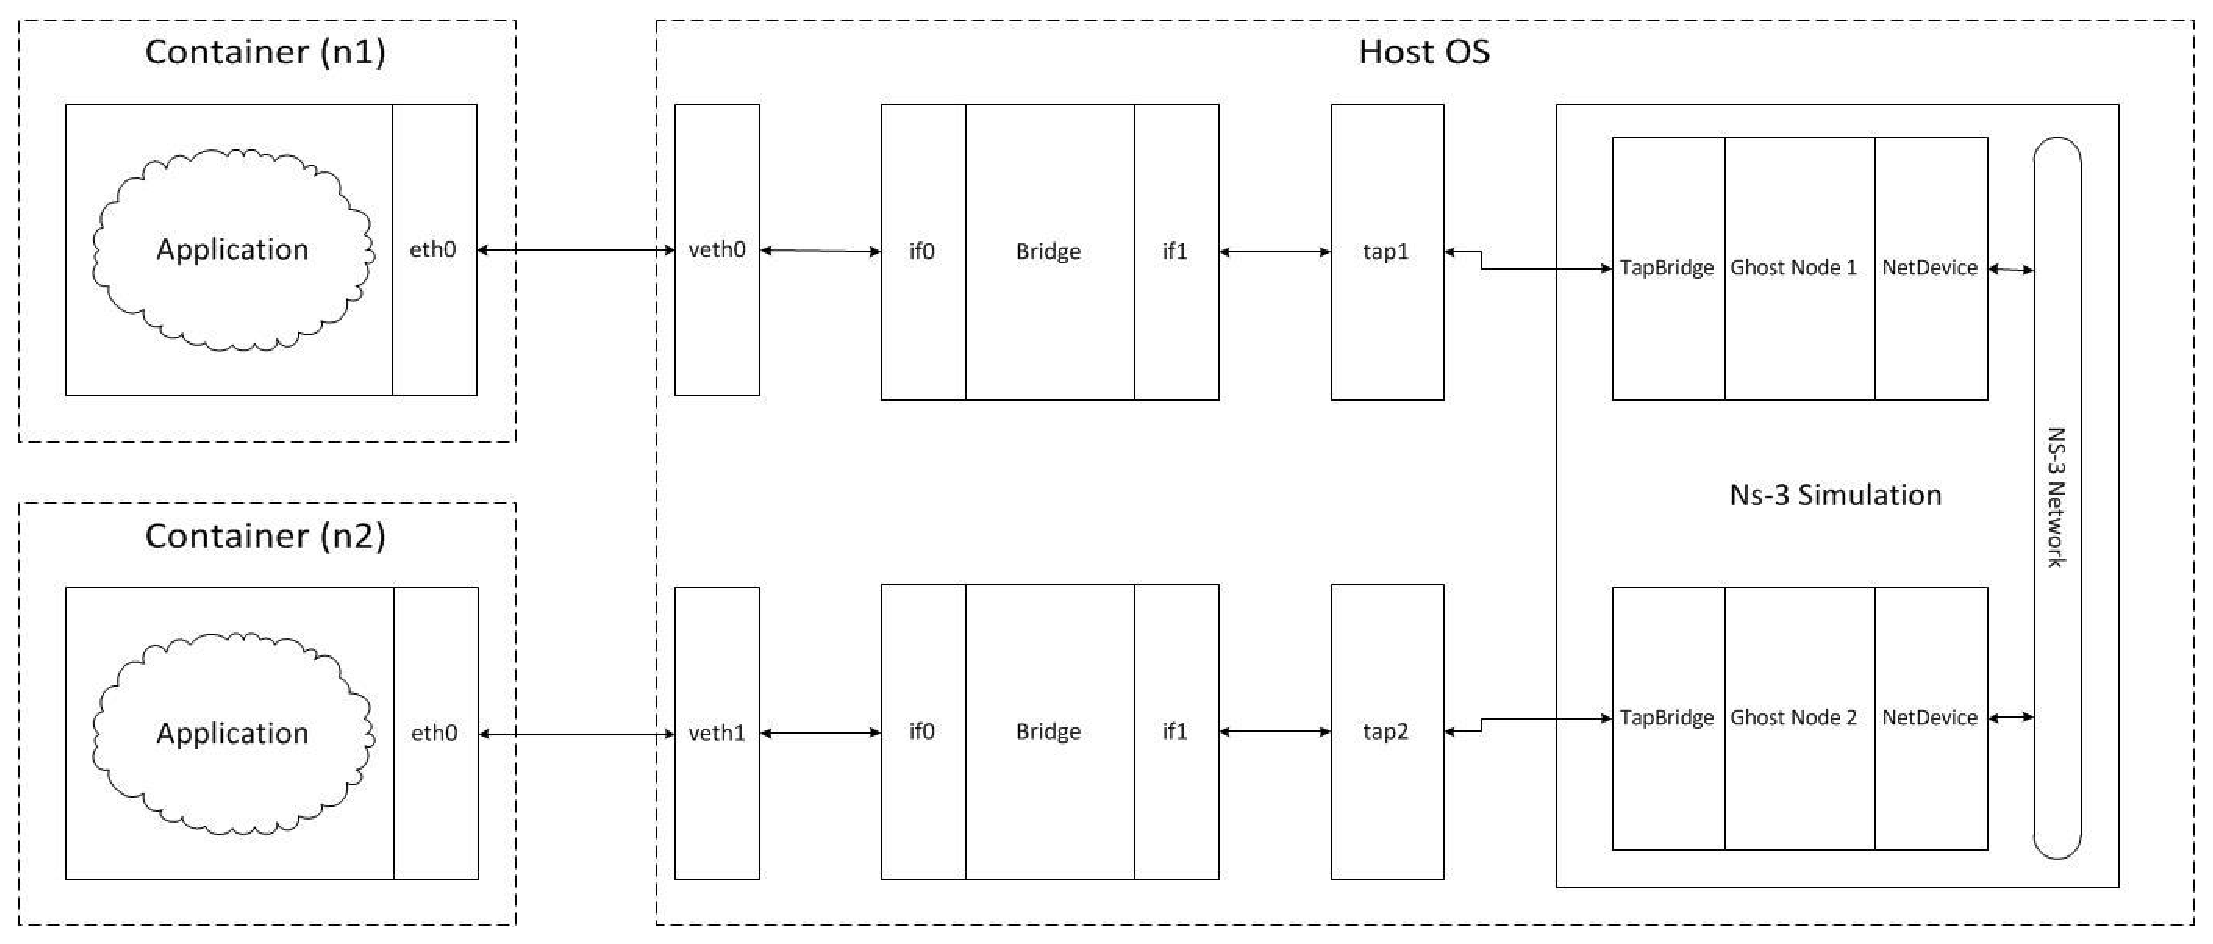
\includegraphics[width=\textwidth]{images/ns3internals.eps} 
    \caption{Connecting LXCs to ns-3} 
    \label{fig:ns3internals}
  \end{figure}
        \end{itemize}
\subsection{NS-3 Modifications}
Integrating TimeKeeper with ns-3 was actually surprising simple. In fact, no changes needed to be made to the ns-3 source code to allow for integration with TimeKeeper! This is because the ns-3 simulator is simply a process with a number of threads. In addition, the RealTime Scheduler utilizes the $gettimeofday()$ system call to determine how far away the simulation time is from the system time. Therefore,  all that is necessary is to add the ns-3 process to the synchronized experiment and assign it a TDF. Then, ns-3's notion of simulation time will progress at the same rate as the other LXCs in the experiment, keeping all of the virtual times synchronized.
